\documentclass[conference]{IEEEtran}
% The following line is only needed to identify funding in the first footnote. If that is unneeded, please comment it out.
\usepackage{amsmath,amssymb,amsfonts}
\usepackage{algorithmic}
\usepackage{graphicx}
\usepackage{textcomp}
\usepackage{xcolor}
\usepackage{float}

\floatstyle{boxed} 
\restylefloat{figure}

\def\BibTeX{{\rm B\kern-.05em{\sc i\kern-.025em b}\kern-.08em
    T\kern-.1667em\lower.7ex\hbox{E}\kern-.125emX}}
\begin{document}

\title{Workshop 2: System Design for Detecting Sleep States Using Accelerometers}
\title{\IEEEoverridecommandlockouts Workshop 2: System Design for Detecting Sleep States Using Accelerometers}
\author{
	\IEEEauthorblockN{Juan Carlos Quintero Rubiano}
	\IEEEauthorblockA{Code: 20232020172\\
		\textit{Systems Engineering} \\
		\textit{Francisco Jose de Caldas District University}\\
		Bogota, Colombia \\
		jcquineror@udistrital.edu.co}\\
	\IEEEauthorblockN{Juan Felipe Wilches Gomez}
	\IEEEauthorblockA{Code: 20231020137\\
		\textit{Systems Engineering} \\
		\textit{Francisco Jose de Caldas District University}\\
		Bogota, Colombia \\
		jfwilchesg@udistrital.edu.co}
	\and
	\IEEEauthorblockN{Juan Nicolas Diaz Salamanca}
	\IEEEauthorblockA{Code: 20232020059\\
		\textit{Systems Engineering} \\
		\textit{Francisco Jose de Caldas District University}\\
		Bogota, Colombia \\
		jndiazs@udistrital.edu.co}
}

\maketitle

\begin{abstract}
	This document builds upon the systemic analysis conducted in Workshop 1 for the Kaggle competition "Child Mind Institute - Detect Sleep States." The focus is on designing a robust system to detect sleep states using accelerometer data. Key findings from the previous analysis, including constraints, data characteristics, and chaos-theory factors, are summarized to guide the design process. The proposed design aims to address identified weaknesses and optimize system performance.
\end{abstract}

\begin{IEEEkeywords}
	System design, sleep state detection, accelerometers, chaos theory, optimization.
\end{IEEEkeywords}

\section{Introduction}
\subsection{Overview of Workshop 1 Findings}
The systemic analysis conducted in Workshop 1 provided a comprehensive understanding of the system for detecting sleep states using accelerometer data. The following key findings were identified:

\begin{itemize}
	\item \textbf{Constraints:}
	      \begin{itemize}
		      \item Sleep periods must be at least 30 minutes long, with interruptions no longer than 30 minutes.
		      \item Only the longest sleep window per night is recorded.
		      \item Device removal periods are not annotated, introducing potential gaps in data.
	      \end{itemize}
	\item \textbf{Data Characteristics:}
	      \begin{itemize}
		      \item The dataset includes accelerometer data with features such as \texttt{anglez} and \texttt{enmo}, which are critical for detecting sleep states, and a \texttt{timestamp} column for time-based analysis.
		      \item Labels for sleep onset and wake events are provided, enabling supervised learning approaches.
	      \end{itemize}
	\item \textbf{Chaos-Theory Factors:}
	      \begin{itemize}
		      \item Sensitivity to initial conditions: Small variations in accelerometer data can lead to significant changes in sleep state classification.
		      \item Randomness in sleep patterns: External factors such as environmental conditions and individual differences introduce unpredictability.
	      \end{itemize}
\end{itemize}

\subsection{Insights from Systemic Analysis}
The systemic analysis provided the following critical insights for designing the system:

\begin{itemize}
	\item \textbf{Feature Importance:}
	      \begin{itemize}
		      \item The accelerometer features \texttt{anglez} and \texttt{enmo} are pivotal for detecting sleep states. Proper preprocessing, such as normalization and noise filtering, is essential to maximize their utility.
		      \item The \texttt{timestamp} column enables time-series analysis, which is crucial for capturing temporal dependencies in sleep patterns.
	      \end{itemize}

	\item \textbf{Handling Data Gaps:}
	      \begin{itemize}
		      \item Device removal periods and unannotated gaps in the data introduce missing values that require robust imputation techniques or strategies to handle incomplete data effectively.
		      \item Strategies such as forward-filling, interpolation, or machine learning-based imputation can be explored to address these gaps.
	      \end{itemize}

	\item \textbf{Temporal Dependencies:}
	      \begin{itemize}
		      \item Sleep states are inherently sequential and time-dependent. Leveraging models designed for time-series data, such as Long Short-Term Memory (LSTM) networks or Temporal Convolutional Networks (TCNs), can improve classification accuracy.
		      \item Capturing transitions between sleep and wake states is critical for accurate predictions.
	      \end{itemize}

	\item \textbf{Model Robustness:}
	      \begin{itemize}
		      \item The system must account for sensitivity to initial conditions, as small variations in accelerometer data can lead to significant changes in classification outcomes.
		      \item Randomness in sleep patterns, influenced by external factors such as environmental conditions or individual variability, requires the model to generalize well across diverse scenarios.
		      \item Techniques such as data augmentation, ensemble modeling, and robust validation can help improve model reliability.
	      \end{itemize}

	\item \textbf{Optimization Goals:}
	      \begin{itemize}
		      \item The design should focus on minimizing false positives (e.g., misclassifying wake states as sleep) and false negatives (e.g., missing sleep onset events) to ensure high precision and recall.
		      \item Computational efficiency is critical, especially if the system is intended for real-time or large-scale deployment.
	      \end{itemize}
\end{itemize}

\section{Requirements Definition}

Based on the initial analysis and the context of the Kaggle competition "Child Mind Institute - Detect Sleep States", the following requirements have been identified for the system design.

\subsection{Translation of Analysis Findings into Design Requirements}

The findings from the systemic analysis are translated into concrete design requirements, covering both functional and non-functional aspects.

\subsubsection{Functional Requirements}
\begin{itemize}
	\item \textbf{Sleep State Detection:} The system must accurately detect sleep and wake states from accelerometer data.
	\item \textbf{Segregation of Longest Sleep Periods:} The system must identify and segregate the longest sleep periods, which must be at least 30 minutes long, as explained in the constraints.
	\item \textbf{Event Annotation:} The system must identify and annotate sleep onset and wake events.
	\item \textbf{Data Gap Handling:} The system should handle missing or incomplete data due to device removal or recording gaps.
\end{itemize}

\subsubsection{Non-Functional Requirements}
\begin{itemize}
	\item \textbf{Performance:} The system should process data with low latency (e.g., response time under 1 second for real-time use) and handle large volumes of time-series data efficiently.
	\item \textbf{Reliability:} The system must achieve high accuracy in sleep state classification (e.g., precision and recall above 90\%) and tolerate occasional data loss or noise.
	\item \textbf{Scalability:} The architecture should allow for scaling to accommodate more users or increased data volume without significant performance degradation.
	\item \textbf{Interpretability:} The system should provide transparent and understandable explanations for its predictions to support clinical and research decision-making.
	\item \textbf{Privacy and Ethics:} The system must ensure data privacy and comply with relevant regulations (e.g., GDPR), especially considering the sensitive nature of children's health data.
	\item \textbf{Adaptability:} The system should be flexible to support studies in different environments and populations, enabling personalized interventions.
\end{itemize}

\subsubsection{Requirements Prioritization}
Requirements are classified as follows:
\begin{itemize}
    \item \textbf{Essential:} Sleep state detection, real-time processing, high accuracy, data privacy.
    \item \textbf{Desirable:} Advanced data gap handling, scalability for large-scale deployment.
    \item \textbf{Optional:} Integration with external health platforms, customizable alerting features.
\end{itemize}

\subsubsection{Requirements Documentation}
All functional and non-functional requirements are documented in a clear and measurable way to ensure they are verifiable during system validation.
\paragraph{Functional Requirements Verification}
\begin{itemize}
    \item \textbf{Sleep State Detection:} Accuracy will be measured using metrics such as precision, recall, and F1-score. The system must achieve at least 90\% precision and recall on a validation dataset.
    \item \textbf{Segregation of Longest Sleep Periods:} The system will be tested on a dataset with annotated sleep periods. It must correctly identify and segregate the longest sleep period in at least 95\% of cases.
    \item \textbf{Event Annotation:} The system's ability to annotate sleep onset and wake events will be evaluated against ground truth labels. A minimum accuracy of 90\% is required.
    \item \textbf{Data Gap Handling:} The system will be tested with datasets containing simulated gaps. It must impute or handle missing data without reducing classification accuracy below 85\%.
    \item \textbf{Event Detection AP Metric:} The system will be evaluated using the competition's Average Precision (AP) metric for event detection. It must achieve a high AP score by accurately matching predicted events to ground-truth events within the specified tolerance thresholds.
\end{itemize}

\paragraph{Non-Functional Requirements Verification}
\begin{itemize}
    \item \textbf{Performance:} The system's processing time will be measured. It must process data with a response time under 1 second for real-time use and handle datasets of up to 1 million rows without significant performance degradation. Additionally, the system must comply with competition constraints, ensuring that CPU or GPU notebooks complete execution within 9 hours.
    \item \textbf{Reliability:} The system will undergo stress testing with noisy and incomplete datasets. It must maintain classification accuracy above 75\% under these conditions.
    \item \textbf{Scalability:} The system will be deployed in a simulated environment with increasing user loads. It must scale to support at least 1,000 concurrent users without exceeding a 5\% increase in response time.
    \item \textbf{Interpretability:} The system will be evaluated by domain experts for its ability to provide clear and understandable explanations for predictions. At least 80\% of experts must rate the explanations as satisfactory or better.
    \item \textbf{Privacy and Ethics:} Compliance with GDPR and other relevant regulations will be verified through an audit. The system must pass all privacy and security checks.
    \item \textbf{Adaptability:} The system will be tested with datasets from different populations and environments. It must maintain accuracy above 85\% across all scenarios.
    \item \textbf{Submission Compliance:} The system must generate a submission file named \texttt{submission.csv} that adheres to the competition's requirements. The notebook must run without internet access and use only freely and publicly available external data, including pre-trained models.
\end{itemize}


\subsubsection{Discussion of Stakeholder Needs}
The system must align with the needs of stakeholders, including:
\begin{itemize}
	\item \textbf{Use Cases:} Support for clinical research, patient monitoring, and large-scale sleep studies.
	\item \textbf{Interpretability:} Provide transparent results and explanations for detected sleep states.
	\item \textbf{Security and Privacy:} Ensure compliance with data protection regulations and ethical standards.
\end{itemize}

The valuable insights generated by this system can inform the development of personalized interventions and support systems tailored to the unique needs of each child, ultimately improving sleep awareness and health outcomes.

\section{High Level Architecture}
The next diagram illustrates the high-level architecture of the system, detailing the basic flow data over the elemets.
\subsection{Diagram Architecture}
\begin{figure}[H]
    \centering
    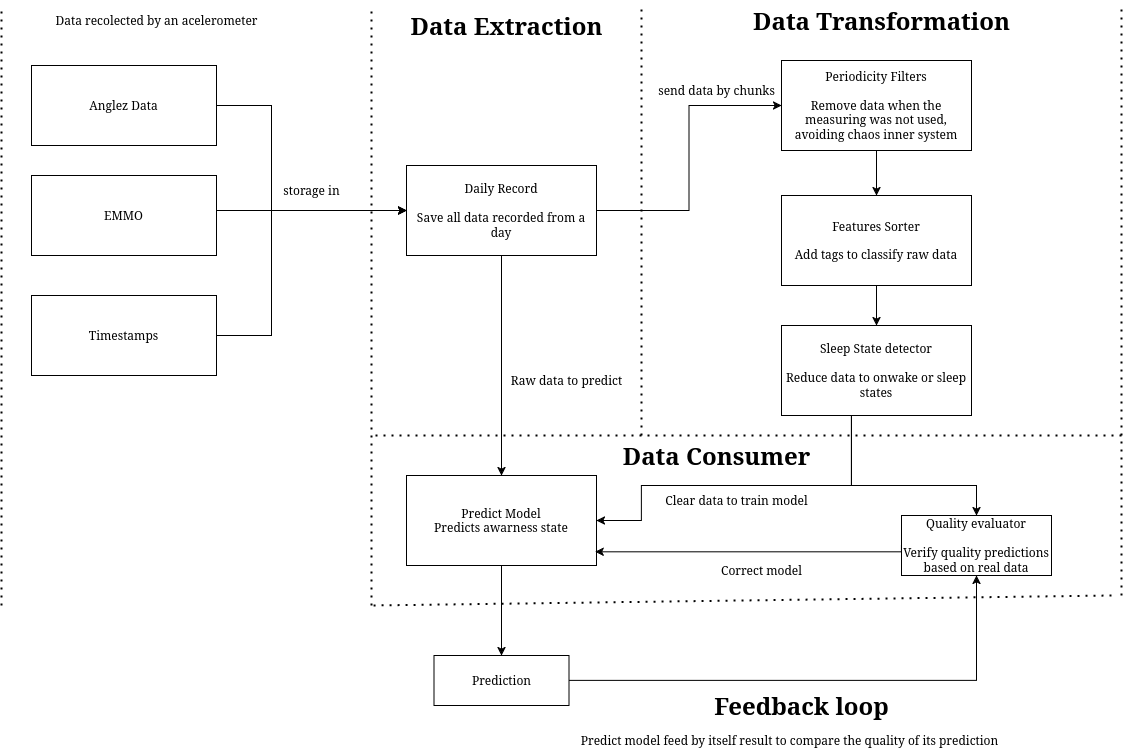
\includegraphics[width=\linewidth]{system.drawio(1).png}
    \caption{System Diagram}
\end{figure}
\subsection{System Engineering principles}
The system is architecure is designed taking into account a holistic view of the processing data flow and elements involved, divided by the following stages:
\begin{itemize}
	\item  \textbf{Data Extraction:} Environment entries are collected from the accelerometer, which is the main source of data for the system. The data is storage into chunks of one day.
	\item \textbf{Data Transformation:} Data is preprocessed to remove noise and irrelevant information by caothic filtering as unnecesary data from device removal periods. The data is then transformed into a format suitable for analysis, including feature extraction.
	\item \textbf{Data Consumer:} Data is consumed by stakeholders to define the sleep state between onwake or sleep. Along side, machine learning model is trained to detect sleep states based on the processed data. The model is evaluated and optimized in a feedback 
	loop which the outputs, predicitions made by the model, return to the system and verify how it is closed the model to the expected value.  
\end{itemize}

\section{Addresing sensitivity and chaos}

The design of the proposed system must take into account the high sensitivity and chaotic nature of sleep state detection.

These manifest themselves in the form of non-linear transitions between sleep and wake states, individual variability, and susceptibility to small perturbations in the accelerometer input.

These challenges arise due to:
\begin{itemize}
\item Non-linear and unpredictable transitions between sleep and wake states.
\item High variability between individuals.
\item Sensitivity to minor fluctuations or noise in sensor inputs, which result in erroneous classifications.
\end{itemize}

To address these complexities, the system integrates robust preprocessing, noise-resilient modeling, and error-handling strategies, ensuring reliable and consistent performance even under uncertain or adverse conditions.

\subsection{Managing High Sensitivity and Chaotic Factors}

\begin{itemize}

\item \textbf{Advanced Data Preprocessing:}
The system applies a pipeline of techniques to reduce the impact of erratic input behavior:
\begin{itemize}
\item Normalization: Ensures that input sequences like anglez and enmo operate on comparable scales, preventing deviations from arbitrary value ranges.
\item Smoothing and Noise Filtering: Implements moving average filters and low-pass filters to suppress spurious spikes or sudden noise while preserving temporal dynamics crucial for detecting sleep transitions.
\item Outlier Detection: Identifies and isolates outliers using statistical thresholds (Z-score, IQR) or anomaly detection models to avoid misleading the learning algorithm.

\end{itemize}

\item \textbf{Robust Sequential Modeling:}  
To capture the time-dependent and non deterministic nature of sleep behavior, the system utilizes:
\begin{itemize}
    \item Long Short-Term Memory (LSTM) Networks: Capable of learning long-range dependencies and distinguishing between transient movements and true state changes.
    \item Temporal Convolutional Networks (TCNs): Offer efficient, parallelizable alternatives to RNNs, with the ability to model long sequences and handle temporal variability.
\end{itemize}

\end{itemize}

\subsection{Monitoring and Error Handling for Unanticipated Conditions}

Due to the unpredictability of real world data like device malfunction, removal of the sensor, or behavioral anomalies, the system incorporates comprehensive mechanisms to monitor, detect, and respond to unexpected issues.
\begin{itemize}
\item \textbf{Real-Time Monitoring Module:}
Continuously scans incoming data streams for:

\begin{itemize}
\item Temporal anomalies: Gaps or irregularities in timestamps that indicate potential data loss.
\item Signal anomalies: Unlikely accelerometer values (constant zero values, data saturation) or flat patterns that may suggest device disconnection.
\item Behavioral anomalies: Unusually long periods of inactivity or hyperactivity inconsistent with typical sleep patterns.
\end{itemize}

\item \textbf{Error Mitigation Routines:}
When detecting irregularities, the system triggers defined recovery strategies such as:
\begin{itemize}
    \item Contextual Imputation: Fills missing or corrupted segments based on neighboring patterns or statistical expectations.
    \item Confidence Suppression: Temporarily reduces classification confidence or halts predictions until data quality is restored.
    \item Soft Degradation: Switches to simpler heuristics (rule based estimation) when machine learning output becomes unreliable due to excessive noise.
\end{itemize}

\item \textbf{Logging and Alerting Mechanism:}
All detected anomalies and actions taken are registered in a structured error registry. Optional alerts are issued when:
\begin{itemize}
    \item A threshold number of anomalies is exceeded in a time window.
    \item High severity conditions (device failure) are detected.
    \item Prediction reliability drops below a critical threshold.
\end{itemize}
This ensures early awareness and intervention by clinicians or researchers, preserving system transparency and integrity.
\end{itemize}
\subsection{Adaptive Learning and Continuous Improvement}

To further enhance resilience against chaos and variability:
\begin{itemize}
\item \textbf{Periodic Model Retraining:} Incorporates newly labeled data from diverse users and conditions to continually refine model robustness.
\item \textbf{Feedback Loops:} Allows expert correction of misclassified events, feeding back into the training pipeline for progressive learning.
\end{itemize}

\section{Technical Stack and Implementation Sketch:}

\subsection{Recommended Tools, Frameworks, and Programming Languages}

To address the challenges associated with detecting sleep states using accelerometer data and to ensure accurate modeling of temporal patterns, the following technology stack is proposed:

\begin{itemize}
\item \textbf{Python:}Chosen for its versatility and wide adoption in data science and machine learning tasks. Python provides extensive support for time series analysis and deep learning through well maintained libraries.
\item \textbf{Pandas and NumPy:} These libraries are essential for data preprocessing and numerical operations, including handling missing values, filtering noise, and feature engineering.

\item \textbf{SciPy and Scikit-learn:}Used for statistical analysis, model evaluation, and classical machine learning approaches like Random Forest or Gradient Boosting to compare against deep learning models.

\item \textbf{TensorFlow Keras or PyTorch:}Deep learning frameworks used to build and train models such as Long Short Term Memory (LSTM) or Temporal Convolutional Networks (TCNs), which are appropiate for learning sequential patterns in time series data.

\item \textbf{Matplotlib and Seaborn:} Visualization libraries used to understand signal trends, explore temporal behaviors, and analyze model performance.

\item \textbf{Jupyter Notebooks:}Ideal for exploratory data analysis, rapid prototyping, and documentation in the development phase.

\item \textbf{Parquet and CSV format support:} Essential for efficiently handling large scale time series datasets in the provided competition structure.
\end{itemize}

These tools are selected for their strong community support, modularity, and effectiveness in handling noisy, chaotic data—key considerations derived from the systemic and chaotic nature of sleep data as analyzed in Workshop 1.

\subsection{Integration and Implementation Plan with Design Patterns}

The system is designed as a modular pipeline composed of independent but interrelated components, adhering to the Pipeline and Strategy design patterns for flexibility and maintainability.

\begin{itemize}
\item \textbf{Data Processor:} Implements the Strategy pattern to allow interchangeable preprocessing strategies (smoothing filters, normalization techniques). Receives raw data and outputs clean time series segments.
\item \textbf{Feature Extractor:} Uses custom functions or sklearn pipelines to compute useful features (moving averages, standard deviation, activity windows).

\item \textbf{Model Selector:} Applies the Strategy pattern to dynamically choose between classical machine learning models or deep learning architectures based on validation performance and interpretability needs.


\item \textbf{Event Detection Module:} Encapsulated as a component that consumes model predictions and transforms them into structured sleep event sequences. Employs thresholding or sequence labeling to identify transitions.

\item \textbf{Validation Module:} Implements the Observer pattern to monitor output events and trigger reprocessing or flag inconsistencies if constraints (minimum 30 minute sleep period) are violated.

\item \textbf{Export Module:}Converts validated events into the final CSV output format with prediction confidence scores, ensuring compatibility with Kaggle evaluation protocol.
\end{itemize}

\textbf{Workflow Summary:}

\begin{enumerate}
\item The Data Processor receives the data raw and applies the appropriate transformation strategy(normalization, noise filtering, data smoothing).
\item Processed data is passed to the Feature Extractor and optionally to a deep learning model through the Model Selector.
\item Predictions are handled by the Event Detection Module, which identifies sleep and wake events.

\item These are verified by the Validation Module, ensuring constraints are met and filtering unreliable results.

\item The final outputs are structured and exported through the Export Module.
\end{enumerate}

This modular design enhances re usability and enables the system to evolve as new data or modeling requirements emerge. It also supports robustness against chaos and sensitivity, as each component can be individually tested and refined without disrupting the entire pipeline.

\end{document}